\section{Compressed Sensing with Coordinate Descent\\ and the direct Fourier Transform}\label{cd}
Instead of using the Major Cycle architecture and approximate the non-uniform FFT approximation, we directly use the Fourier transform matrix $F$. We show the principle of our approach and of Compressed Sensing reconstructions in general at a simplified example. Let us minimize the objective function \eqref{cd:clean}.

\begin{equation}\label{cd:clean}
\underset{x}{minimize} \: \left \| V - Fx \right \|_2^2 + \lambda \left \| x \right \|_1 \\
\end{equation}

The data term $\left \| V - F^{-1}x \right \|_2^2$ forces our image to be similar to the measurements, and the regularization term $\left \| x \right \|_1$ tells us how likely the current reconstruction is to be the true image. The parameter $\lambda$ weights the trade-off between the data and the regularization term. With our term we assume our image contains only a limited number of non-zero pixels.  When the instrument observes stars, they take up a single pixel in the image. In this case, our prior models the true image well, and the theory of compressed sensing states we are virtually guaranteed to find the truly observed image at the minimum of our objective function \eqref{cd:clean}.

We can use a number of different optimization algorithms to optimize \eqref{cd:clean}. Note however in the one dimensional case, where we only have one pixel, the data term of the objective \eqref{cd:clean} forms a parabola and the regularization term a shrink operation\footnote{The shrink operation reduces the magnitude of the pixel by $\lambda$. For example: Pixel $x = -12.4$, $\lambda = 0.6$. The new pixel value after shrinkage follows as $shrink(-12.4, 0.6) = -11.9$}. The optimum for a single pixel can be calculated by solving for the minimum of the parabola first, followed by a shrink operation. With Coordinate Descent we can exploit this property. We fix all pixels except for one and iteratively solve for the current minimum of each pixel. Now when we iterate over all pixels several times, we eventually converge to a solution. The full Coordinate Descent algorithm can be implemented in a few lines of python code:

\begin{lstlisting} 
def coordinate_descent(V_residual, x, lambda, max_iter):
	for k in range(0, max_iter):
		for i in pixels_row:
			for j in pixels_column:
				x_old = x[i, j]
				fourier_column = calculate_fourier_transform(i, j)
				fr = real(fourier_column)
				fi = imag(fourier_column)
				rr = real(V_residual)
				ri = imag(V_residual)
				
				#find apex
				a = sum(fr**2 + 2*fr*fi + fi**2)
				b = sum(fr*rr + fr*ri + fi*rr + fi*ri)
				x_new = b / a + x_old
				
				x_new = shrink(x_new, lambda)
				x[i, j] = x_new
				V_residual = V_residual - fourier_column * (x_new - x_old)
\end{lstlisting}\label{cd:basic}

Coordinate Descent has to iterate over every pixels possibly several times. How quickly Coordinate Descent converges in theory is not well understood. Our optimization function \eqref{cd:clean} falls in the class of quadratic programming with a strictly convex objective. In this case, Coordinate Descent is guaranteed to converge at least linearly\cite{luo1992convergence}. Sadly, real-world objective functions for image reconstruction are often not strictly convex. Usually our image is constrained to have only positive pixels\cite{mcewen2011compressed}, which breaks the strictly convex property of the objective function. In our environment, the convergence guarantees of Coordinate Descent are not well understood in theory.

In practice, Coordinate Descent can be improved with heuristics. Since we assume our image contains only a few stars, a few non-zero pixels, the simple Coordinate Descent algorithm wastes resources checking if the pixel is still zero. A better scheme would be the active set heuristic\cite{friedman2010regularization}: We iterate over every pixel once. Then, for a given number of iterations, we only check the pixels that have changed. This is an improvement, but too expensive in the context of MeerKAT. A reconstruction problem can have billions of Visibilities and serveral millions of pixels. Since $F$ has the size of Visibilities times pixels, it gets too expensive to calculate all columns even once.

However, it turns out we do not need to if we imitate CLEAN: For CLEAN, the non-uniform FFT approximates the 'dirty' image, which is corrupted by the effects of incomplete measurements. CLEAN then subtracts a fraction of the PSF at the largest pixel value. In other words, the largest pixel value in the dirty image is the most likely non-zero pixel. We can use the dirty image approximation for a 'probability distribution' of non-zero pixels. It does not need to be accurate, since the actual reconstruction is done with the direct Fourier Transform.

This is, in principle, how the proof-of-concept algorithm works. Instead of reconstructing an image, it reconstructs in the starlet space. It uses the starlet transform of the dirty image to find likely non-zero components. Coordinate Descent is used to optimize single starlets. A proof-of-concept version of this algorithm was developed in python.

Although the algorithm produces super-resolved images in section \ref{results}, it is currently not known if it actually converges to the true optimum. Finding all relevant non-zero starlets is left to a greedy heuristic. There may be conditions under which it never includes relevant components. Further convergence analysis was outside the scope of the project. Also note that for this implementation, every time likely non-zero components are searched, it simply uses the non-uniform FFT for the dirty image approximation. This was done for simplicity's sake and can be improved.


\subsection{The Starlet Transform} \label{cd:starlets}
First we introduce the starlet transform, and then describe how we use it to estimate likely non-zero starlet components.

\begin{figure}[h]
	\centering
	\begin{subfigure}[b]{0.4\linewidth}
		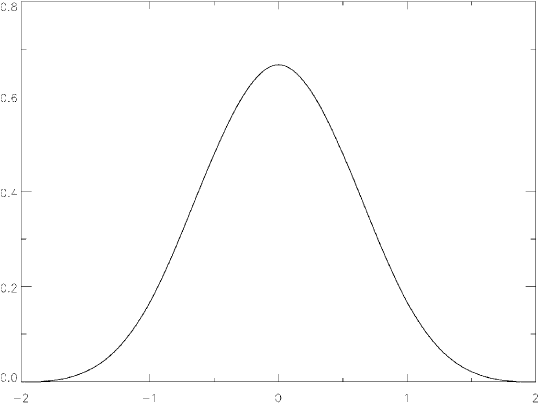
\includegraphics[width=\linewidth]{./chapters/05.algorithms/starlets/scaling.png}
		\caption{Spline scaling function}
		\label{cd:starlets:scaling}
	\end{subfigure}
	\begin{subfigure}[b]{0.4\linewidth}
		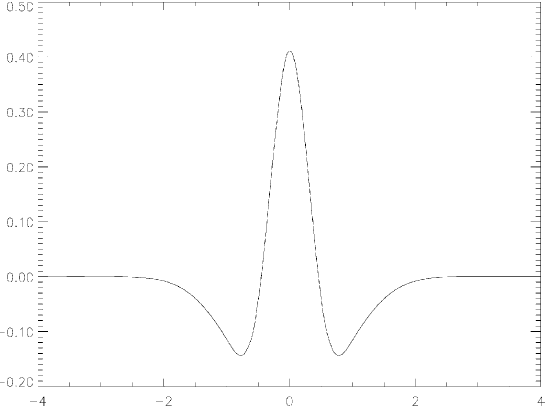
\includegraphics[width=\linewidth]{./chapters/05.algorithms/starlets/wavelet.png}
		\caption{Wavelet function}
		\label{cd:starlets:wavelet}
	\end{subfigure}
	\caption{Scaling and wavelet function of the starlet wavelet. Source: \cite{starck2015starlet}}
	\label{cd:starlets:figure}
\end{figure}

The starlet transform is an Isotropic Undecimated Wavelet Transform (IUWT) with the starlet wavelet shown in figure \ref{cd:starlets:figure}. It defines two operations: The transformation from starlet into image space which is called synthesis, and the inverse which is called decomposition. The starlet space represents an image in multiple layers at different scales, where lower layers contain smaller objects and upper layers the extended emissions. The lowest starlet layer represents the stars, while the upper layer represents the widest hydrogen clouds in the image.

\begin{equation}\label{cd:starlet:w0}
\begin{aligned}
	c_0 &= \bm{x} \star B_0 \\
	\bm{w_0} &= \bm{x} - c_0
\end{aligned}
\end{equation}

Let us look at the lowest starlet layer first, how it is calculated from the image, and how we use it for image reconstruction. The starlet layer $w_0$ gets calculated in two steps, shown in \eqref{cd:starlet:w0}. First, we take the scaling function for the lowest layer $B_0$, and convolve the image with it, resulting in the blurred image $c_0$. The blurring removes the smaller structures of the image. In the last step, we subtract the blurred image $c_0$ from $x$ and arrive at the starlet layer 0, $w_0$. It contains the smallest structure of the image convolved with the starlet wavelet. 

This is where the starlet transform ends. Note that we do not get the actual starlet components $\alpha_0$ for the layer. The transformation just decomposes the structures of the image into layers. The actual starlet components $\alpha_0$ would be the result of a deconvolution. 

\begin{figure}[h]
	\centering
	\begin{subfigure}[b]{0.25\linewidth}
		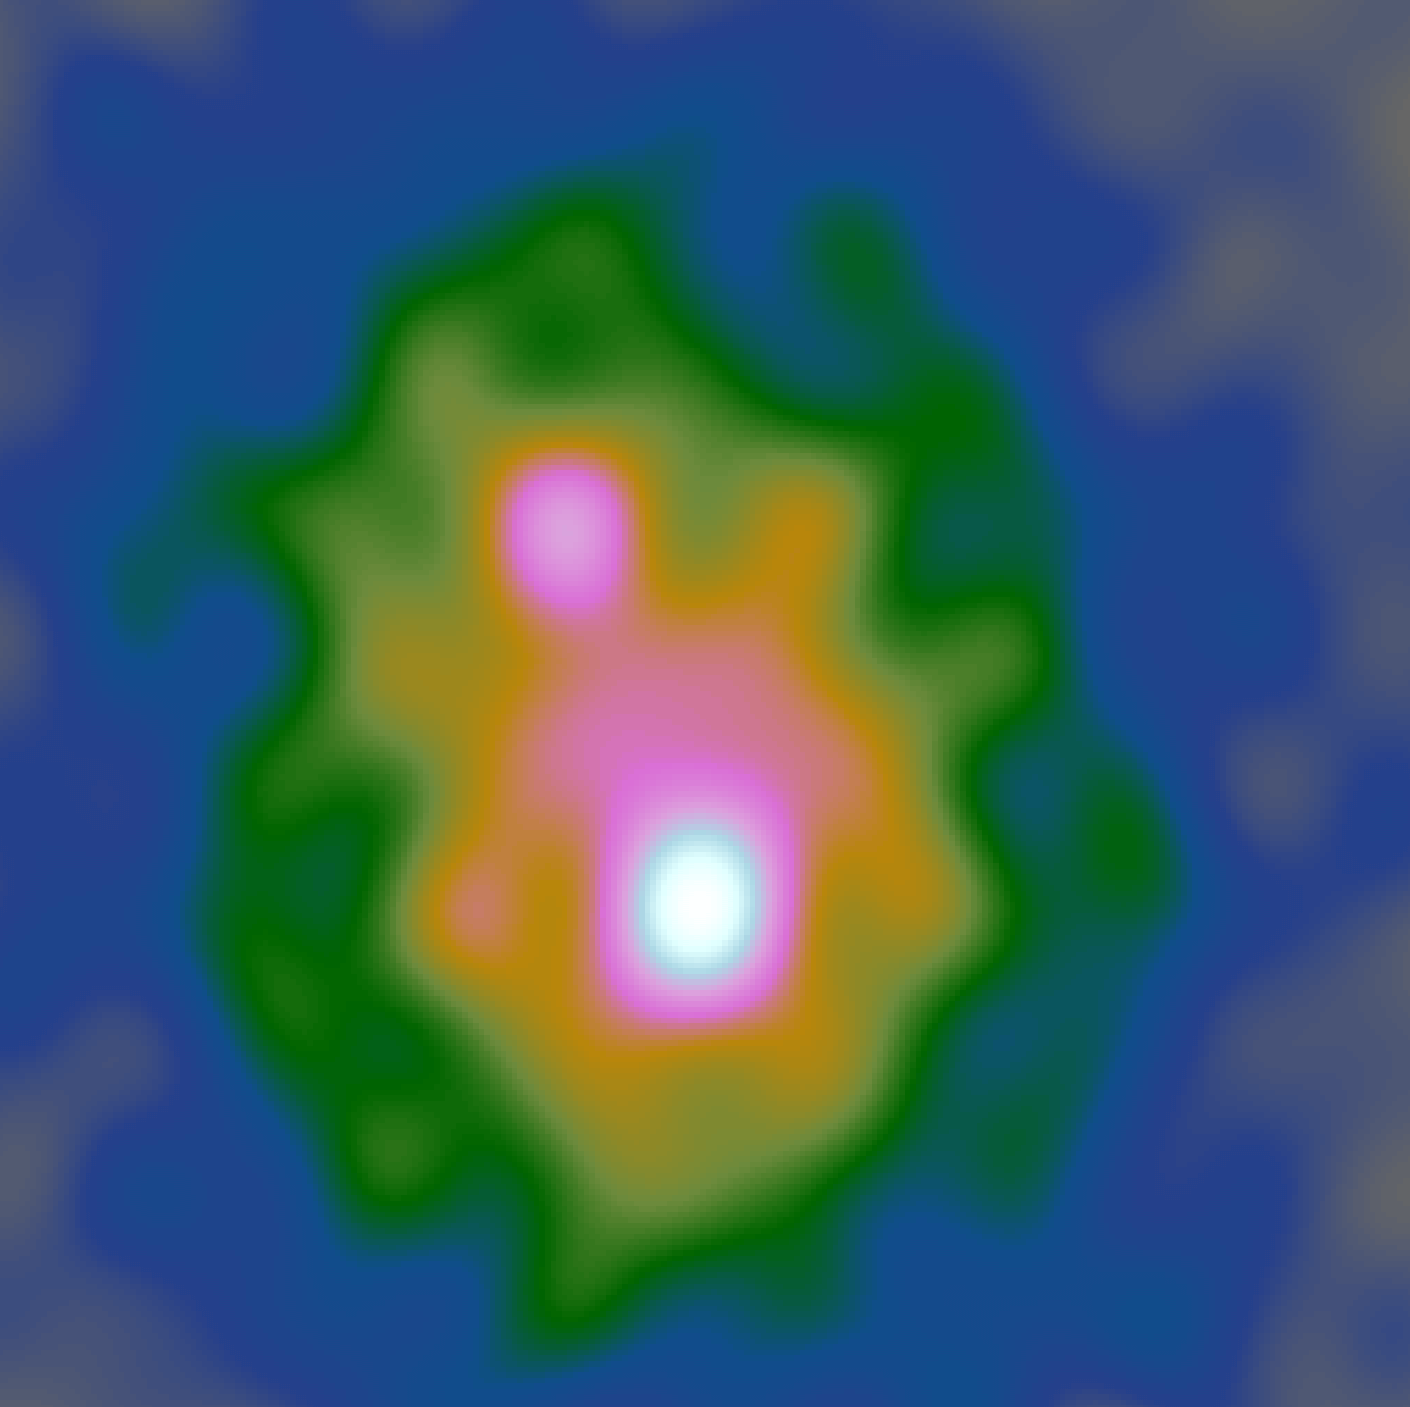
\includegraphics[width=\linewidth]{./chapters/05.algorithms/starlets/dirty2.png}
		\caption{Dirty Image with two point sources.}
		\label{cd:heuristic:dirty}
	\end{subfigure}
	\begin{subfigure}[b]{0.25\linewidth}
		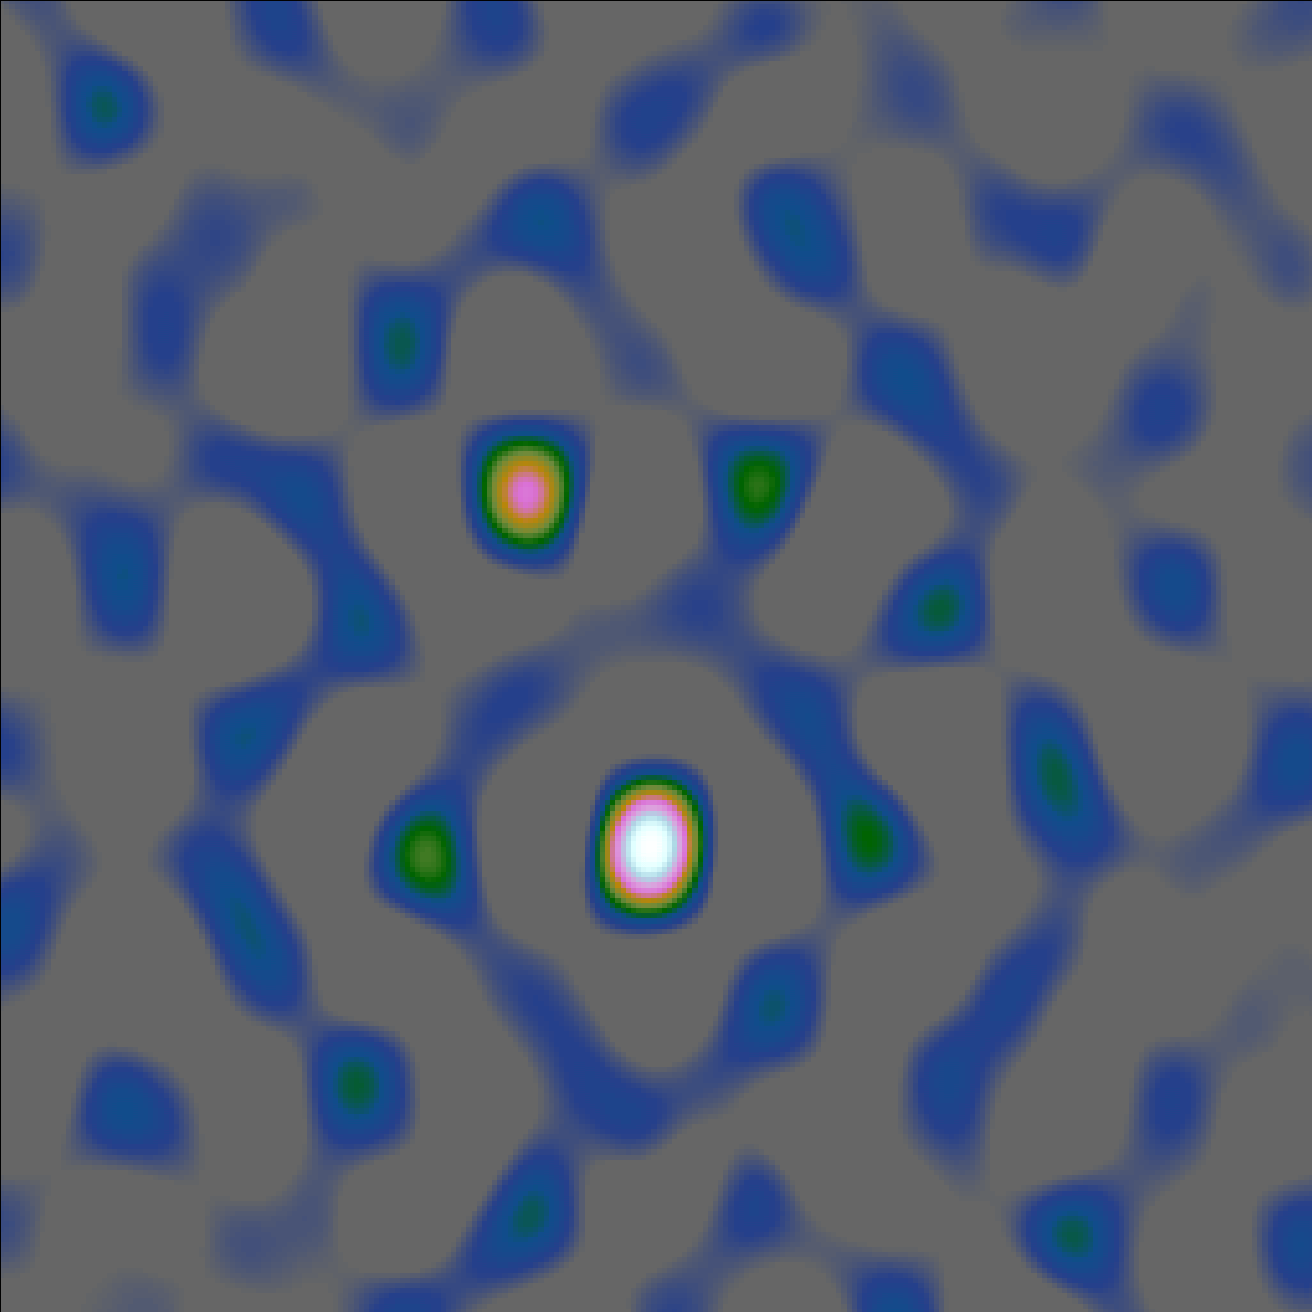
\includegraphics[width=\linewidth]{./chapters/05.algorithms/starlets/starlet0_2.png}
		\caption{Layer $w_0$ of the starlet decomposition.}
		\label{cd:heuristic:starlet}
	\end{subfigure}
	\caption{Dirty map and $w_0$ starlet layer after shrinkage. $w_0$ can be interpreted as a probability distribution for point source locations.}
	\label{cd:heuristic:figure}
\end{figure}

It turns out we can estimate the starlet components $\alpha_0$ by simply shrinking the starlet layer $w_0$. Figure \ref{cd:heuristic:figure} shows an example of the process. Coordinate Descent will reconstruct the image with starlet components $\alpha_0$, but it does not need to try all components. We use the starlet transform as a heuristic and can estimate likely non-zero $\alpha_0$.

The same process is repeated for all $J$ layers. We calculate the starlet decomposition shown in equation \eqref{cd:starlet:decomposition}. We continually blur the image with ever wider scaling functions $B_i$. We subtract the more heavily blurred image $ c_{J-1}$ from $c_{J-2}$ to arrive at the starlet layer, which contains the structures of the current size $w_{J-1}$. The scaling function $B_i$ widens exponentially, and the top level starlet spans an area of $5*2^{J-1}$ pixels. Note that the last starlet layer is the most blurred version of the image $c_J$. It contains all structures which were wider than the widest starlet.

\begin{equation}\label{cd:starlet:decomposition}
\begin{split}
c_0 &= \bm{x} \star B_0 \\
\bm{w_0} &= \bm{x} - c_0
\end{split}
\qquad
\begin{split}
c_1 &= c_0 \star B_1 \\
\bm{w_1} &= c_0 - c_1
\end{split}
\qquad \ldots \qquad
\begin{split}
c_{J-1} &= c_{J-2} \star B_{J-1} \\
\bm{w_{J-1}} &= c_{J-2} - c_{J-1}
\end{split}
\qquad
\begin{split}
\bm{c_J} &= c_{J-1} \star B_J
\end{split}
\end{equation}

We shrink all the starlet layers $w_i$ and $c_J$, and arrive at which components $\alpha_i$ are likely non-zero. Coordinate Descent converges on the optimal $\alpha_i$ for all layers. At this point, we can reconstruct the image by reversing the process. We convolve $\alpha_i$ with the starlet wavelet at scale i, which gives us $w_i$. Then, we sum them up to the final image \eqref{cd:starlet:backwards}.

\begin{equation} \label{cd:starlet:backwards}
\bm{x} = \bm{w_0} + \bm{w_1} + \ldots + \bm{w_{J-1}} + \bm{c_J}
\end{equation}

This is how we  leverage the starlet transform for our Coordinate Descent algorithm. Note that we can use the starlet transform as a heuristic without necessarily using the starlet components $\alpha_i$ for reconstructions. The starlet transform gives us likely locations of Gaussian-shaped emissions at different scales. We can for example use a Gaussian mixture model, and just use the starlets for likely non-zero locations. 

In this work, we do not use the wavelet shown in image \ref{cd:starlets:wavelet}. Instead, we modified the starlet to an extend where it arguably is not a wavelet any more. Still, the starlet transform with the correct wavelet as a heuristic, but reconstructed the image with a modified starlet to satisfy the non-negativity constraint. 


\subsubsection{Non-negative Starlet Modification}\label{cd:starlets:modification}
Reconstruction algorithms for Radio Astronomy typically constrain the image to be non-negative\cite{mcewen2011compressed}. We can constrain the starlet components $\alpha_i$ to be non-negative, but the starlet wavelet has negative sections. Which leads to negative areas in the layers $w_0$, and negative pixel values in the reconstructed image $x$.

The simple fix is to either set all negative pixels of $x$ to zero, or to set negative values of $w_i$ to zero. Both lead to slightly different artefacts in the $x$, and both do not lead to significantly better results.

For reconstruction, we modify the starlet wavelet and set all negative sections to zero. At this point, the reconstruction starlet is arguably not a wavelet any more, since its integral is larger than zero. But now the Coordinate Descent algorithm can reconstruct a non-negative image which has led to a more sparse representation of images in the next section.



\subsection{Coordinate Descent Implementation}
In this section, we put together the starlet transform and the Coordinate Descent to form our algorithm. We use two separate loops of Coordinate Descent minimization. First, let us look at the objective function \eqref{cd:starlet:layer} for a single starlet layer and discuss why we still need the non-uniform FFT for pre-calculation. 

Our target is to use as few columns from $F$ as possible. As we have seen in equation \eqref{cd:starlet:decomposition}, each starlet is a series of convolutions. We can also do the convolution in Fourier space, and we only need to calculate the columns of $F$ for non-zero starlets instead of non-zero pixels. This leads us to the following objective \eqref{cd:starlet:layer} for a single layer $i$.

\begin{equation}\label{cd:starlet:layer}
\underset{\alpha_i}{minimize} \: \left \| V - S_iF\alpha_i \right \|_2^2 + \lambda \left \| \alpha_i \right \|_1 \\
\end{equation}

The drawback is that we need to calculate all the convolutions for the starlets at layer $i$ in the non-uniformly sampled Fourier space. We used the non-uniform FFT approximation to calculate all $S_i$. This introduces an approximation again. In the future, one can find the optimal $S_i$ in the non-uniform Fourier space by solving an optimization problem similar to objective \eqref{killmajor:sep:major}. The starlet is constant for a given observation, which means we can pre-calculate all $S_i$ before the optimization. 


\subsubsection{Iteration Scheme and Heuristics}
Our algorithm is split in two separate Coordinate Descent loops. The first "adding" loop, iterates over the starlet components of a single layer. Here  we use the starlet transform as a heuristic and add likely non-zero components. The second, "sparsifying" loop iterates over all non-zero components of all layers. Together they form one full iteration of our proof-of-concept algorithm.
\begin{lstlisting} 
def one_full_iteration(V_residual, alpha, J, lambda):
	#adding loop
	for j in reverse(range(0, J)):
		a = alpha[j]
		active_set = starlet_decomposition(non_uniform_fft(V_residual), lambda)
		a = coordinate_descent(V_residual, active_set, lambda, 10)
		
	#sparsifying loop
	non_zero = sum(abs(alpha))
	for i in range(0, 10):
		for j in range(0, J):
			a = alpha[j]
			active_set = a[non_zero > 0]
			a = coordinate_descent(V_residual, active_set, lambda, 1)
\end{lstlisting}\label{cd:full}

The adding loop minimizes the objective \eqref{cd:starlet:layer}. We first use the starlet transform for estimating likely non-zero components. We then use Coordinate Descent and iterate over the likely non-zero components. In theory, the Coordinate Descent iterations in the adding loop are not necessary. The sparsifying loop will converge to the same solution. In practice, the Coordinate Descent iterations help to reduce the non-zero components we add. When we look again at image \ref{cd:heuristic:starlet}, which shows the likely location of point sources, we see that the individual locations are not independent. Coordinate Descent iterations here help to reduce the number of non-zero starlets that get minimized in the sparsifying loop.

The adding loop minimized each layer separately. The task for the sparsifying loop is to minimize $alpha_i$ for all layers. In this implementation, we look at all $\alpha_i$ for each non-zero location in $\alpha$. If the adding loop set a point source at a certain pixel location, the sparsifying loop checks if a wider starlet at the same location minimizes the objective.

Our modified starlet starlet

The starlet transform allows for a myriad of heuristics with Coordinate Descent. In the adding loop, we sort the active set heuristic.We leveraged another fact of the starlet transform 







